%
%  untitled
%
%  Created by Johan Boissard [] on 2010-06-24.
%  Copyright (c) Johan Boissard. All rights reserved.
% hhh

\documentclass[a4paper,titlepage] {scrartcl}
\usepackage[T1]{fontenc}
\usepackage[utf8]{inputenc}
\usepackage{graphicx}
\usepackage{engord}
%\usepackage[english]{babel}
\usepackage{fancyhdr}
\usepackage{amsmath, , amssymb}
\usepackage{comment}

\usepackage{listings}

%allows inclusion of url (hyperref is better than url) 
%ref: http://www.fauskes.net/nb/latextips/
\usepackage{hyperref}

%package for chemistry ie: \ce{(NH4)2SO4 -> NH4+ + 2SO4^2-} 
%ref:www.ctan.org/tex-archive/macros/latex/contrib/mhchem/mhchem.pdf
\usepackage[version=3]{mhchem}
%celsius + degrees
\usepackage{gensymb}
%to get last page
\usepackage{lastpage} % \pageref{LastPage}

%make use of the fullpage (no HUGE margins)
\usepackage{fullpage}
\usepackage{subfig}

%allows separating cell in table by diagonal line
\usepackage{slashbox}




%\renewcommand{\chaptername}{Laboratory}
%\setcounter{chapter}{5}

\usepackage{color}
\usepackage[usenames,dvipsnames, table]{xcolor}
% Include this somewhere in your document



\usepackage[absolute]{textpos}

%column  of multi row in tables
\usepackage{multirow}

%to have vertical text in table
\usepackage{rotating}


%%%%%%% a virer ici!!!!
\begin{comment}
%Fonts and Tweaks for XeLaTeX
\usepackage{fontspec,xltxtra,xunicode}
%\defaultfontfeatures{Mapping=tex-text}
%\setromanfont[Mapping=tex-text]{Hoefler Text}
\setsansfont[Scale=MatchLowercase,Mapping=tex-text]{Gill Sans}

\definecolor{shade}{HTML}{D4D7FE}	%light blue shade
\definecolor{text1}{HTML}{272727}		%text is almost black
\definecolor{headings}{HTML}{173849} 	%dark blue %%%dark red 70111
\definecolor{title}{HTML}{173849} 	%dark blue %%%dark red 70111

\usepackage{titlesec}				%custom \section
\end{comment}







\author{Johan Boissard}
\date{\today}
\title{Econometrics}
\begin {document}

%\maketitle
%\tableofcontents

\section{Intro to statistics and Econometrics}

\paragraph{Empirical analysis} % (fold)
\label{par:empirical_analysis}
economists are forced to use \textbf{observational} data
% paragraph empirical_analysis (end)

\paragraph{Econometrics} % (fold)
\label{par:econometrics}
use \textbf{economic theory} and \textbf{economic data}
% paragraph econometrics (end)

\subsection{Economic data}
\begin{itemize}
	\item cross-sectional data (at one point in time)
	\item time series data (spans an interval)
	\item combining both
\end{itemize}

\subsection{Causality}
correlation $\neq$ causality

\subsection{Probability}
\begin{itemize}
	\item Probability density function (pdf): 
	\begin{equation}
		f_X(x)
	\end{equation}
	\item Joint distribution
	\begin{equation}
		f_{X,Y}(x,y)=f_{Y|X}(y|x)f_X(x)=f_{X|Y}(x|y)f_Y(Y) 
	\end{equation}
	\item conditional distribution
	\begin{equation}
		f_{Y|X}(y|x)=\frac{f_{X,Y}(x,y)}{f_X(x)}
	\end{equation}
\end{itemize}

\subsection{How to summarize a probability distribution} % (fold)
\label{par:how_to_summarize_a_probability_distribution}
\begin{itemize}
	\item Mean
	\begin{equation}
		\mu = \mathbb{E}(X)=\int_{\mathbb R} xf(x)dx
	\end{equation}
	\item Variance
	\begin{equation}
		\sigma^2=\operatorname{Var}(x)=\mathbb E [(X-\mu)^2]=\mathbb E(X^2)-\mu^2
	\end{equation}
	\item Standard deviation 
	\begin{equation}
		\sigma = \operatorname{sd}(X)=\sqrt{\sigma^2}
	\end{equation}
\end{itemize}
% paragraph how_to_summarize_a_probability_distribution (end)

\subsubsection{Important properties}
\begin{eqnarray}
	\mathbb E(c) &=& c\\
	\operatorname{Var}(c)&=&0\\
	\mathbb E(aX+b) &=& a\mathbb E(X) +b\\
	\operatorname{Var}(aX+b) &=& a^2\operatorname{Var}(X)\\
	\mathbb E(aX+bY) &=& a\mathbb E(X) +b\mathbb E(Y)\\
	\operatorname{Var}(aX+bY) &=& a^2\operatorname{Var}(X)+b^2\operatorname{Var}(Y)-2ab\operatorname{Cov}(X,Y)
\end{eqnarray}

if $X$ and $Y$ are independant, then $\operatorname{Cov}(X,Y)=0$.

\subsubsection{Correlation}
\begin{equation}
	\operatorname{Corr}(X,Y) = \frac{\operatorname{Cov}(X,Y)}{\operatorname{sd}(X)\operatorname{sd}(Y)}
\end{equation}

\subsection{Standardized Normal distribution $\mathcal N(0,1)$}

\begin{itemize}
	\item is symmetric
	\item total area $= 1$
	\item $68\%$ of area is comprised between $\pm 1$
	\item $95\%$ of area is comprised between $\pm 2$
\end{itemize}

\paragraph{Each Normal distribution can be converted to the standardized form} % (fold)
\label{par:each_normal_distribution_can_be_converted_to_the_standardized_form}
if
\begin{equation}
	X\sim\mathcal N(\mu, \sigma^2)
\end{equation}
  then 
\begin{equation}
	Z = \frac{X-\mu}{\sigma} \sim \mathcal N (0,1)
\end{equation}
% paragraph each_normal_distribution_can_be_converted_to_the_standardized_form (end)


\subsection{Other distributions}

\subsubsection{$\chi^2$ distribution}
Let $n$ independant variables $Z_i \sim \mathcal N(0,1)$ then	\begin{equation}
	X = \sum_{i=1}^nZ_i^2
\end{equation}
has $\chi^2$ distribution with $n$ degrees of freedom
\begin{equation}
	X \sim \chi_n^2
\end{equation}

\subsubsection{$t$-distribution}

Let $Z\sim\mathcal N(0,1)$ and $X\sim\chi_n^2$
then 
\begin{equation}
	T = \frac{Z}{\sqrt{X/n}}
\end{equation}
has a $t$ distribution with $n$ degrees of freedom.

\subsubsection{$F$-distribution}
Let $X\sim\chi_k^2$ and $Y\sim\chi_l^2$ and assume that $X$ and $Y$ are independant, then 
\begin{equation}
	F = \frac{X/k}{Y/l}
\end{equation}
has an $F$ distribution with $(k,l)$ degrees of freedom.


\subsection{Estimating the population mean}
We wanna know then mean $\mu$ of the population

How good is the sample mean as an estimator for the population mean ?
\begin{itemize}
	\item Point estimator
	\item Confidence interval
\end{itemize}

\subsubsection{Central Limit Theorem}
Let $\{Y_1, ..., Y_n\}$ be a random sample with mean $\mu$ and variance $\sigma^2$.

Then 
\begin{equation}
	Z_n=\frac{\sum Y_i/n-\mu}{\sigma/\sqrt{n}}
\end{equation}
has an asymptotic standard normal distribution


\subsubsection{Law of Large Numbers}
Let $Y_1,...,Y_n$ be independant identically distributed (iid) random variables with mean $\mu$. Then	
\begin{equation}
	\lim_{n\rightarrow\infty}\frac{1}{n}\sum_{i}^nY_i=\mu
\end{equation}


%%% week2 %%%
\section{Simple Regression Analysis}
\begin{equation}
	\mathbf{y} = \beta_0+\beta_1\mathbf{x}+\mathbf{u}
\end{equation}
where
\begin{itemize}
	\item $y$ is the dependent variable
	\item $x$ independent variable
	\item $u$ error or disturbance term
\end{itemize}

\subsection{Assumptions}
\begin{itemize}
	\item SLR1: Linear parameters
	\item SLR2: Zero conditional mean
	\begin{equation}
		\mathbb E(u|x)=\mathbb{E}(u)=0
	\end{equation}
	which implies
	\begin{equation}
		\mathbb E(y|x)=\beta_0+\beta_1x
	\end{equation}
\end{itemize}

\subsection{Slope estimate}
\begin{equation}
	b_1=\frac{\sum_i^n(x_i-\overline x)(y_i-\overline y)}{\sum_i^n(x_i-\overline x)^2}
\end{equation}

\begin{equation}
	\hat u_i=|y_i-\hat y_i|
\end{equation}

\subsection{Derive OLS estimators}
Minimize for $b_0$ and $b_1$
\begin{equation}
	\sum_i(\hat u_i^2)=\sum_i(y_i-b_0-b_1x_i)^2
\end{equation}

\subsubsection{Properties of OLS}
\begin{eqnarray}
	\sum_i\hat u_i&=&0\\
	\sum_ix_i\hat u_i&=&0\\
	\overline y &=& b_0+b_1\overline x
\end{eqnarray}

\subsection{Terminology}
\begin{itemize}
	\item Sum of squares Total 
	\begin{equation}
		SST = \sum_i(y_i-\overline y)^2
	\end{equation}
	\item Sum of squares Exlained
	\begin{equation}
		SSE = \sum_i(\hat y_i-\overline y)^2
	\end{equation}
	\item Sum of squares Residual
	\begin{equation}
		SSR = \sum_i(y_i-\hat y_i)^2= \sum_i(\hat u_i)^2
	\end{equation}
\end{itemize}
\begin{equation}
	SST = SSE + SSR
\end{equation}
\subsection{Goodness of fit $r^2$}
\begin{equation}
	r^2=\frac{SSE}{SST} = 1 - \frac{SSR}{SST}
\end{equation}

\subsection{Functional forms}
\begin{tabular}{cccc}
\hline
model & equation & slope & elasticity\\
\hline
level-level & $y = \beta_0+\beta_1x+u$ & $\beta_1$ & $\beta_1$\\
\hline
level-log & $y = \beta_0+\beta_1\ln(x)+u$ & $\beta_1/x$ & $\beta_1$\\
\hline
log-level & $\ln(y) = \beta_0+\beta_1x+u$ & $\beta_1/y$ & $\beta_1$\\
\hline
log-log & $\ln(y) = \beta_0+\beta_1\ln(x)+u$ & $\beta_1y/x$ & $\beta_1$\\
\hline
\end{tabular}


\subsection{Unbiasedness of OLS}
\begin{eqnarray}
	b_1 &=&  \frac{\sum_i^n(x_i-\overline x)(y_i-\overline y)}{\sum_i^n(x_i-\overline x)^2}
	\\
	&=& \beta_1 + \sum_i^n(x_i-\overline x)\frac{u_i}{SST_x}
	\\
	\mathbb E{(b_1)}&=&\beta_1
	\\
	...
	\\
	\mathbb E(b_0)&=&\beta_0
\end{eqnarray}

\subsection{Homoskedacity}
\begin{equation}
	\operatorname{Var}(u|x)=\operatorname{Var}(u)=\sigma^2
\end{equation}
and we have
\begin{equation}
	\operatorname{Var}(b_1)=\frac{1}{SST_x}\sigma^2
\end{equation}

\subsubsection{Unbiased estimate of the error variance ($\sigma^2$)}
\begin{equation}
	s^2 = \sum_i^n\frac{\hat u_i^2}{n-2} = \frac{SSR}{n-2}
\end{equation}


%% week 2: second part %%%
\section{Multiple Regression}
\begin{equation}
	y= u + \beta_0 +\sum_{i=1}^k\beta_ix_i
\end{equation}
... allows a \emph{ceteris paribus} interpretation

\subsection{Direction of bias}
\begin{tabular}{ccc}
\hline
 & $\operatorname{Corr}(x_1,x_2)>0$ & $\operatorname{Corr}(x_1,x_2)<0$\\
\hline
$\beta_2>0$ & positive bias & negative bias\\
\hline
$\beta_2<0$ & negative bias & positive bias\\
\hline
\end{tabular}

\subsection{OLS variances}
\begin{equation}
	\operatorname{Var}(b_j)= \frac{1}{SST_j(1-r_j^2)}\sigma^2
\end{equation}

%%% week 3 %%%
\section{Multiple Regression Analysis - Further Issues}

\subsection{Tests}
we can test either
\begin{itemize}
	\item two sided
	\item one sided
\end{itemize}
We test:

$H_0: \beta_j=0$ against
$H_1: \beta_j\neq0$
or build a \textbf{confidence interval}.


\subsection{The $F$-test}
Test: $H_0: \beta_1=0, \beta_k=0$, we have
\begin{equation}
	F = \frac{SSR_r-SSR_{ur}}{SSR_{ur}}\frac{n-k-1}{q}
\end{equation}

$F \sim F_{q,n-k-1}$
\begin{figure}[htbp]
	\centering
		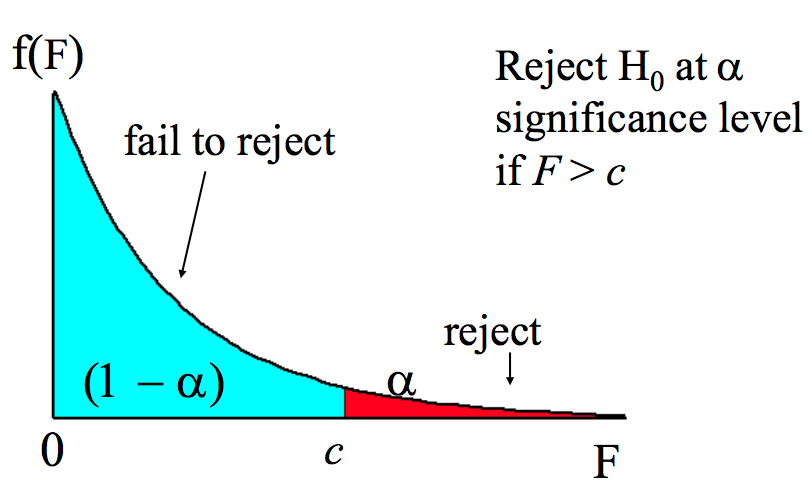
\includegraphics[height=3in]{images/testF.png}
	\caption{Test $F$}
	\label{fig:images_testF}
\end{figure}


\end{document}
